% Chapter 4

\chapter{Experimental setup} % Main chapter title

\label{Chapter4} % For referencing the chapter elsewhere, use \ref{Chapter4}


%----------------------------------------------------------------------------------------

\section{Introduction}
The majority of prediction tools are based on the assumption that it is the miRNA seed region that contains almost all the important interactions between a miRNA and its target and their focus are on these canonical sites.

In this thesis, we aim at using deep learning techniques to investigate the role of those non-canonical sites and pairing beyond the canonical seed region in miRNA targets. Recent increases in computational power have permitted the rise of methods that can dispense with human-crafted features, making it possible to deal directly with raw data and autonomously learn and identify patterns to appropriately represent it. In particular, deep learning has been shown to be an effective method for classification tasks in domains with complex feature representation \cite{dl}.

Deep Learning (DL) has already been applied to the miRNA target prediction problem. Cheng et al. \cite{mirtdl} used convolutional neural networks to analyze matrices of miRNA:site features, but the selected features were still human-crafted descriptors and thus the method faces similar problems as rule-based and ML approaches. A more recent work, DeepTarget \cite{deep_target}, relied on recurrent neural networks to identify potential binding sites and assess their functionality. However, this work is still oriented to the identification of canonical sites and relies on a limited small data set for the training phase. Another approach using DL is DeepMirTarSdA \cite{deep_mirtar}, that explore the use of stacked de-noising auto-encoders (SdA) to predict human miRNA-targets at the site level, but the network obtained is huge and the small availability of input data (about 8000 samples between positives and negatives) results in a model that performs well on the data being used but generalizes quite poorly. 

In this thesis, we present DeepMiRNA, a miRNA target prediction tool that attempts to exploit the learning capacity of a neural network to extract abstract patterns from raw input data. Unfortunately, to the best of our knowledge, there is no suitable raw-data representational method for miRNA-target prediction. This is very likely the consequence of the very small quantity of validated data available for this task. For this reason, rather than making an assumption about suitable descriptors, we created a set of rules to help finding the best candidate binding sites leaving the classification decision to the neural network (see CSSM in the next section). 

More precisely, DeepMiRNA scans the 3'UTR of the gene identifying potential target sites according to the chosen rules. It then uses the previously trained network to identify the relevant patterns by directly examining the whole mature miRNA transcript, rather than focusing on the seed region and analyzing precomputed descriptors. In the following text, we denote a miRNA binding site with MBS.

\section{Preparing for training}
Two of the fundamental properties in deep neural network theory states that:

\begin{enumerate}
	\item with sufficient data samples and a correct network design a NN can approximate any mathematical function
	\item a NN has the capacity to automatically learn the relevant features of complex data structures by means of its hidden layers \cite{dl}
\end{enumerate}

For these reasons, in our approach we sought to minimize potential biases introduced by handcrafted features by working with the miRNA and the mRNA transcripts, feeding them directly to the neural network.

The DeepMiRNA working pipeline for the identification of functional targets for miRNAs can be summarized as follows (Figure \ref{fig:pipeline}: a 30-nucleotide sliding window with a stride of 5 nucleotides is used to scan the 3'UTR of a given gene. Both values (size and stride) have been empirically computed during the training stage (see the results section for more information). For each mRNA 30-nucleotide long subsequence, the VIENNA RNACofold package \cite{vienna_rna} is used to compute the stability of the binding between the miRNA transcript and the fragment. If the computed value is below a predetermined threshold, the primary structure of the mRNA and the miRNA are examined to see if the criteria defined by the candidate site selection rules (CSSR) are met. If so, the duplex is vectorized and fed into the network for classification. The prediction is then further refined using an a posteriori filter that computes the site accessibility of the mRNA region surrounding the predicted binding site. 

In the next two sections, we will describe how DeepMiRNA's neural network actually comes in two different flavors according to the encoding algorithm used: either one feed-forward (also called Multi Layer Perceptron MLP) or one convolutional network.
 
We pointed this out because, despite the important role of site accessibility in miRNA target identification described in recent articles \cite{accessibility_nrg_role} \cite{common_features}, the filtering stage has only been used with the convolutional neural network. This decision has been made according to the experimental results obtained: the MPL model, in fact, exhibited great ability in identifying negative binding sites correctly. The filtering step does not significantly increase the model's performance while it slows down the testing process, hence we opted for its exclusion.

The situation changes when the convolutional network is employed for the task: for this model site accessibility has revealed an important role in false positive reduction, justifying the decision to keep the filtering stage with this configuration. More details about this feature can be found in section \ref{sub:filtering_step}.    

\begin{figure}[hbt!]
	\centering
	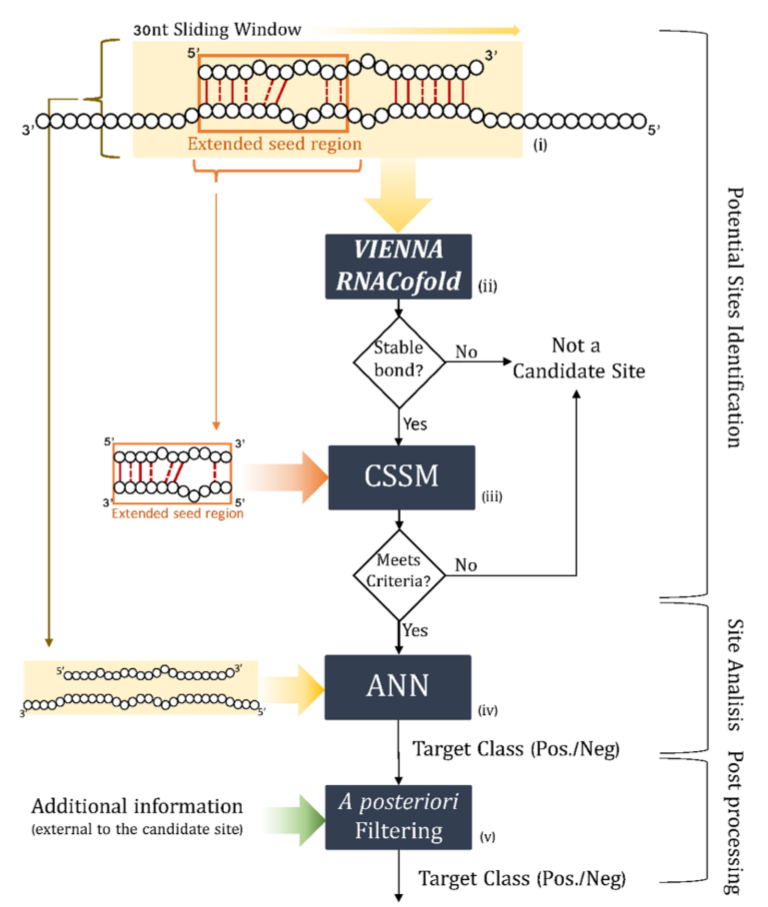
\includegraphics[width=0.8\textwidth]{Figures/pipeline}
	\caption{\textbf{DeepMiRNA pipeline}. (i) a 30nt sliding window with a 5nt step is used to scan the gene transcript; (ii) The Vienna Cofold software is used to compute the binding stability; (iii) if the bond is predicted to be stable a partial complementarity according to the rules defined in the CSSR is verified; (iv) if all previous checks passed the duplex is fed to the NN for prediction; (v) for positive predictions a filter is used to compute the site accessibility of the miRNA: if the energy needed to access the site is above a certain threshold the prediction is changed to negative.}
	\label{fig:pipeline}
\end{figure}

\subsection{Data preprocessing}
A key factor for successful application of any Machine Learning technique and one of the most important aspects to consider before feeding the network with data is how we prepare the input data and the targets.  

The main aspect to consider during this process is the use of suitable techniques to make the data more amenable for the NN: this includes vectorization, normalization and handling of missing values. 

\subsubsection{vectorization}
In order to be accepted by the neural network, all inputs must be tensors, that is they must be expressed by numerical arrays with suitable shape and dimension. The process to encode categorical data, in our case the transcript sequences, into tensor is called \emph{vectorization}. In this thesis we actually employed two different techniques for this operation: 

\begin{itemize} 
	\item one hot encoding of the sequences \cite{onehotencode}. 
	\item sequence embedding using a Word2Vec approach \cite{word2vec}. 
\end{itemize}

One hot encoding is a process by which categorical data such as strings are converted into binary vectors. In our case, each nucleotide is translated to a binary vector of size 4, corresponding to the four possible nucleotide values as described in Table \ref{tab:ohe} 

\begin{table}[!b]
	\caption{One Hot encoding of a nucleotide.}
	\label{tab:ohe}
	\centering
	\begin{tabular}{l l}
		\toprule
		\tabhead{Nucleotide} & \tabhead{Encoding} \\
		\midrule
		A & [1, 0, 0, 0]\\
		C & [0, 1, 0, 0]\\
		G & [0, 0, 1, 0]\\
		U or T & [0, 0, 0, 1]\\
		Empty & [0, 0, 0, 0]\\
		\bottomrule
	\end{tabular}
\end{table}

The main problem using this method is that not all duplexes have the same size. This is in particular due to the different miRNA's transcript length (ranges from 18 to 30), The network, instead, requires that all inputs have the same shape. Hence, in order to meet this requirement, every miRNA sequence, when needed, has been padded with 'empty' letters to reach the maximum size length (in this case 30). Regarding the site transcript, each fragment has a size of 40: 30 corresponding to the window size plus 5 additional nucleotides upstream and downstream. These additional nucleotides seek to capture any influence that the flanking sequence may exert on the target \cite{conserved_pairing}. With these adjustments, each duplex is represented by a binary vector of (fixed) size 280.

The second vectorization method uses a Word2Vec approach. Whereas the vectors obtained through one-hot encoding are binary and sparse (mostly made of zeros), sequence embeddings are usually dense, very low-dimensional floating-point vectors. 

Word2Vec \cite{word2vec} is a Natural Language Processing (NLP) methodology to map words into numeric vectors based on their context. Being the context defined as the words surrounding the word to encode. For DNA sequences, however, there is no clear definition for words, so usually, a kmer (that is a set of $k$ continuous nucleotides)is used to define a word (see Figure \ref{fig:dna2vec}). Therefore, in case of biological sequences, the context is defined as the set of $n$ adjacent kmers (being $n$ a parameter to validate). For this thesis use the software available at \url{https://github.com/pnpnpn/dna2vec} to train the model used to encode the kmers. This encoding has two important advantages compared to one hot encoding:

\begin{enumerate}
	\item each kmer of length comprised between 3 and 8 is mapped to an equal size vector of size 100.
	\item similar kmers are mapped to close points in the features space according to a specific distance metric (usually Euclidean distance).
\end{enumerate}

In our case, each variable length miRNA sequence has been split into 4 different size kmers each mapped into a 100-dimension vector, while each fixed size site transcript (plus the flanking nucleotides) has been split into 5 8-mers. This way each duplex is mapped into a $9x100$ matrix obtained concatenating the resulting 9 vectors. It's important to note that this vectorization requires a different design and implementation of the neural network to use as we will describe in the next section.

\begin{figure}[hbt!]
	\centering
	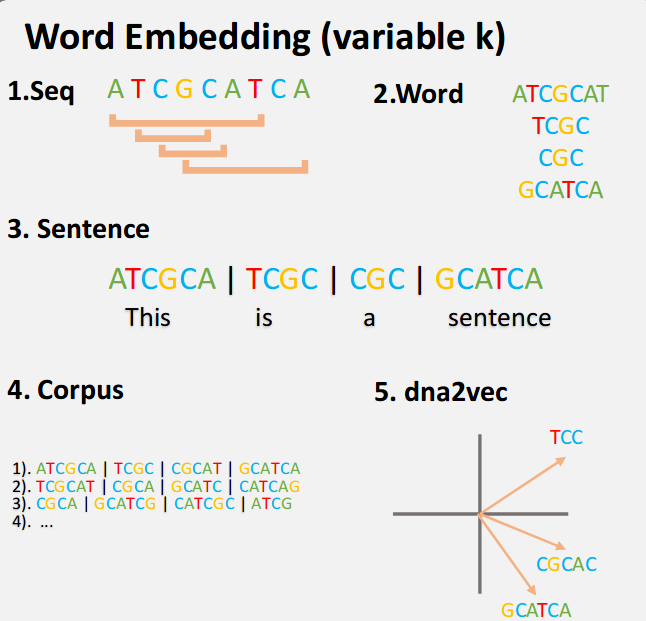
\includegraphics[width=0.7\textwidth, height=0.3\textheight]{Figures/dna2vec}
	\caption{Dna2Vec mapping example using different length k-mers}
	\label{fig:dna2vec}
\end{figure}

\subsubsection{normalization and missing values}
Another crucial part of data preprocessing concerns their normalization. In general, it's not safe to feed the network with data that takes relatively large values or that are heterogeneous (i.e have very different values ranges). In our case, however, the vectorization process guarantees that the numerical values resulting from the encoding are both small and homogeneous. Regarding missing or incomplete data, we found a very small quantity of them in the datasets retrieved, hence we simply decided to discard them.  

\subsection{Dataset preparation}
One of the biggest challenges to face in any Machine Learning application is to get a good set of significant data.
The main purpose is to have a sufficiently variable and representative dataset that allows the model to generalize well on new and unseen examples. This phase is probably the most important together with the network design as it's crucial for achieving good performances. It is of fundamental importance that the data is representative of the problem we want to solve. It does not matter how big is the quantity of data we obtain if that is not aligned with the goal we want to pursue. One should focus on finding data with features that matter to what we’re trying classify or predict and discard unrelated features. Hence, the first step of a classification process should be proper data collection, and until we achieve this, we will find ourselves constantly coming back to this step \cite{imbalanced_datasets}.

For the miRNA target prediction task, this requires a comprehensive dataset of verified positive and negative targets that encompass both canonical and non-canonical examples. While there are multiple data repositories providing information regarding experimentally validated positive miRNA targets\cite{dianatarbase} \cite{mirtarbase}, there are significantly fewer experimentally verified negative targets. This represents a major concern for ML-based approaches that require similar numbers of labeled examples for both classes.

In this thesis we only considered human data and we used the version 8 of the Diana TarBase\footnote{\url{http://diana.imis.athena-innovation.gr/DianaTools/index.php}} and the release 7.0 of miR TarBase\footnote{\url{http://mirtarbase.mbc.nctu.edu.tw/php/index.php}} datasets. Moreover, in order to annotate the datasets with lacking informations such as molecules transcripts, we downloaded gene sequences from Ensembl\footnote{\url{https://ensembl.org/index.html}} and miRNA transcripts from miRBase\footnote{\url{http://mirbase.org}} 

\subsubsection{Diana TarBase}
Diana TarBase is the most widely used database for validated miRNA interactions. The latest version at the time of writing is $v8$ and asking for a bulk download from their website is possible to obtain a dataset of 526658 positive and 63559 negative validated targets. This dataset provides information about miRNA:mRNA interactions in the form of miRNA name, gene name and functionality as it's illustrated in Table \ref{tab:Diana}. Unfortunately, there is no information about transcript sequences of the molecules or binding sites location.

\begin{table}[!t]
	\caption{Example of Diana TarBase entries.}
	\label{tab:Diana}
	\centering
	\begin{tabular}{l l l}
		\toprule
		\tabhead{gene name} & \tabhead{miRNA name} & \tabhead{functionality} \\
		\midrule
		AB002442 & hsa-miR-192-5p & POSITIVE\\
		DAD3R & hsa-miR-34a-5p & NEGATIVE\\
		E2IG4 & hsa-miR-200c-3p & POSITIVE\\
		\bottomrule
	\end{tabular}
\end{table}

\subsubsection{Mir TarBase}
This database contains interactions of about 2000 miRNA and around 20000 genes. In total the downloaded dataset comprises 380091 positive and 382 negative duplexes available from the Download section of the website. It's possible to find it under the name \textit{hsa\_MIT.xlsx}. It's important to note that every single miRNA can interact with hundreds of different genes. Again, exactly as with the Diana TarBase dataset, no sequence or binding sites transcripts are provided.
 
\subsubsection{Ensembl}
From Ensembl\cite{ensembl} is possible to obtain the transcripts of all human genes. In our work, we focused on the 3'UTR and for the download we used the BioMart tool available from the main menu. More specifically, from the BioMart webpage, we followed these steps:
\begin{itemize}
	\item from the drop down menu choose database: \emph{Ensembl Genes 96};
	\item then choose dataset: \emph{human genes GRCh38.p12};
	\item from the left-hand side of the page click attributes and select \emph{sequences};
	\item from this submenu select \emph{3'UTR} and then click on \emph{Header Information};
	\item now from the header submenu select the following attributes: \emph{Gene stable ID}, \emph{Gene name}, \emph{Transcript stable ID}, \emph{3'UTR start} and \emph{3'UTR end};
	\item lastly click on \emph{Results} from the top left and export the generated fasta file selecting the box \emph{Unique results only} and pressing \emph{Go}.
\end{itemize}
Note that a single gene identified with a unique ID may produce multiple RNA's transcripts each denoted with its own transcript ID. The actual transcript observed will depend on the tissue, developmental time point, and environmental or hormonal factor. Typically there's a single major transcript expressed in a given cell at a given time, but not always. Unfortunately in both the Diana TarBase and miR TarBase the transcript ID of the miRNA:mRNA pair is not present, hence, according to what is used in \cite{deep_mirtar}, we kept the transcript with the longest sequence.  

\subsubsection{mirBase}
The mirBase database allowed us to retrieve all known miRNAs transcripts. For the homo sapiens species there currently around 2000 miRNAs sequences and in order to collect them, we followed these steps:
\begin{itemize}
	\item from the homepage click \emph{Browse} from the top menu;
	\item click on \emph{human} and a preview of the data will appear on screen as depicted in figure \ref{fig:mirna_preview};
	\item on the bottom of the page select sequence type \emph{Mature sequence} and output format \emph{Unaligned fasta format};
	\item press \emph{Select all} and then \emph{Fetch sequences}; 
	\item the query result will be printed on the next page where it can be copied and pasted to a regular text file and saved as a fasta file.
\end{itemize}
 
\begin{figure}[hbt!]
	\centering
	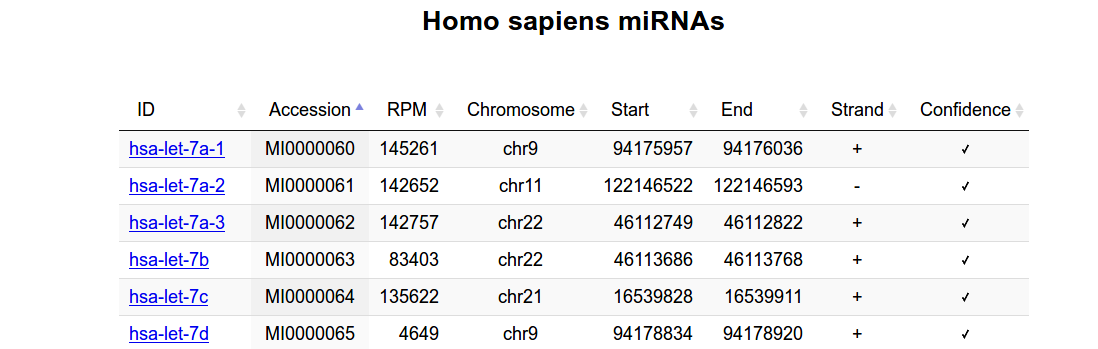
\includegraphics[width=1\textwidth, height=0.3\textheight]{Figures/mirna_preview}
	\caption{A sample of the mirBase database.}
	\label{fig:mirna_preview}
\end{figure}

As a preliminary step, the Diana and Mir TarBase data were parsed to remove inconsistent entries, that were marked both as positive and negative targets due to contradictory results in different experimental validations, and combine entries that were validated more than once by different verification methods. We also filtered pairs were the annotated 3'UTR sequence length was shorter than 200 nucleotides.  This produced a final dataset of 593407 positive (+) and 33604 negative (-) miRNA:mRNA interactions containing bindings for about 16000 different genes and around 2000 miRNAs. This data was then split into two parts for the training and testing phases using a ratio of 67:33, thus obtaining a training functional set of 397582 positives and 22504 negatives and a test set of 195825 positives and 11100 negatives.

\subsection{Training dataset}
Structuring a proper training dataset is an essential aspect of effective deep learning models but one that is particularly hard to solve. Part of the challenge comes from the intrinsic relationship between a model and the corresponding training dataset. If the performance of a model is below expectations, it is often hard to determine whether the causes are related to the model itself or to the composition of the training dataset.

The purpose of this stage is to train and validate the neural network that has the responsibility for distinguishing between functional (positive) and non-functional (negative) target sites. A positive experimentally validated gene can exhibit tens of potential positive binding sites but not necessarily all of them are actually functional. Hence, the training set must be composed of miRNA:MBS pairs rather than miRNA:mRNA duplexes. However, the retrieved data, while consistent and sufficiently various, do not contain such information. Searching the Internet we were able to find only 2 publicly available validated datasets providing information regarding experimentally identified miRNA binding site locations: the Helwak \cite{helwak} and the Grosswendt \cite{grosswendt} datasets.

\subsubsection{Positive binding sites}
The two above datasets contain miRNA:MBS locations obtained through PAR-Clip \cite{parclip}  and CLASH \cite{clash}  experiments, however, the binding site identified might not be functional. Hence, in order to consider a site as positive, we cross-reference them with the Diana TarBase and miR TarBase. In particular, we considered a given duplex miRNA:MBS as functional if:
\begin{itemize}
	\item form a stable bond, that is it has a measure of free energy below a predetermined threshold according to Vienna Cofold. The threshold used was $-10$ $kcal/mol$.+
	\item correspond to a miRNA:gene pair marked as functional in either the Diana or the miR dataset.
\end{itemize} 
Additionally, we complemented our positive training dataset by including the most probable broadly conserved sites obtained from TargetScanHuman 7.1 \cite{targetscan} that matched experimentally validated functional data from Diana Tarbase or mirTarBase.
This process produced a total of 32774 positive miRNA:MBS duplexes for the training stage.

\subsubsection{Negative binding sites}
The small number of non-functional experimentally validated binding sites makes 
the construction of a representative negative dataset a very difficult task. Some of the examined existing tools overcome this issue by creating 'mock' targets \cite{mirmark} continuously shuffling the sequence of a real functional binding site until the resulting transcript does not appear in any positive miRNA target repository. This method, however, may lead the neural network to learn the function used to create the negative examples resulting in a model trained to discriminate between artificial and real data rather than discerning functional targets from non-functional. Besides, there is no guarantee that the generated sequence is indeed a true negative because it has not been experimentally validated.

The solution we implemented opted for using the validated miRNA:mRNA pairs to extract the negative binding sites and add them the ones provided by the CLASH and CLIP experiments. The idea is that any sequence of approximately 30 nucleotides in the mRNA of a negatively validated miRNA:mRNA pair may represent a potential negative target site. However, in order to avoid the introduction of noise including such sequences, we decided to keep only subsequences of mRNA where the associated miRNA has the potential to form a stable bond. In order to check this requirement, we used a sliding window of 30 nt along the entire 3'UTR region. For each negative miRNA:mRNA pair we kept the  MBS with the lowest binding energy. For some pairs, there might be no candidate satisfying the CSSM reequirements, in this case, we just discard the entry. From the 22504 negative pairs of the original training set, we were able to create 22205 negative MBSs (see Figure \ref{fig:training}). The binding energy (or free energy) was  computed according to the RNACoFold function from the RNA library \cite{vienna_rna}. 

\subsubsection{Training stage}
Once the positive and the negative datasets have been created, we shuffled and merged them to create a unique dataset. The whole process of creation of the training set is illustrated in figure \ref{fig:training}. In order to train and validate the network, we kept 80\% of the data for training and the rest for validation and test set. 

\begin{figure}[hbt!]
	\centering
	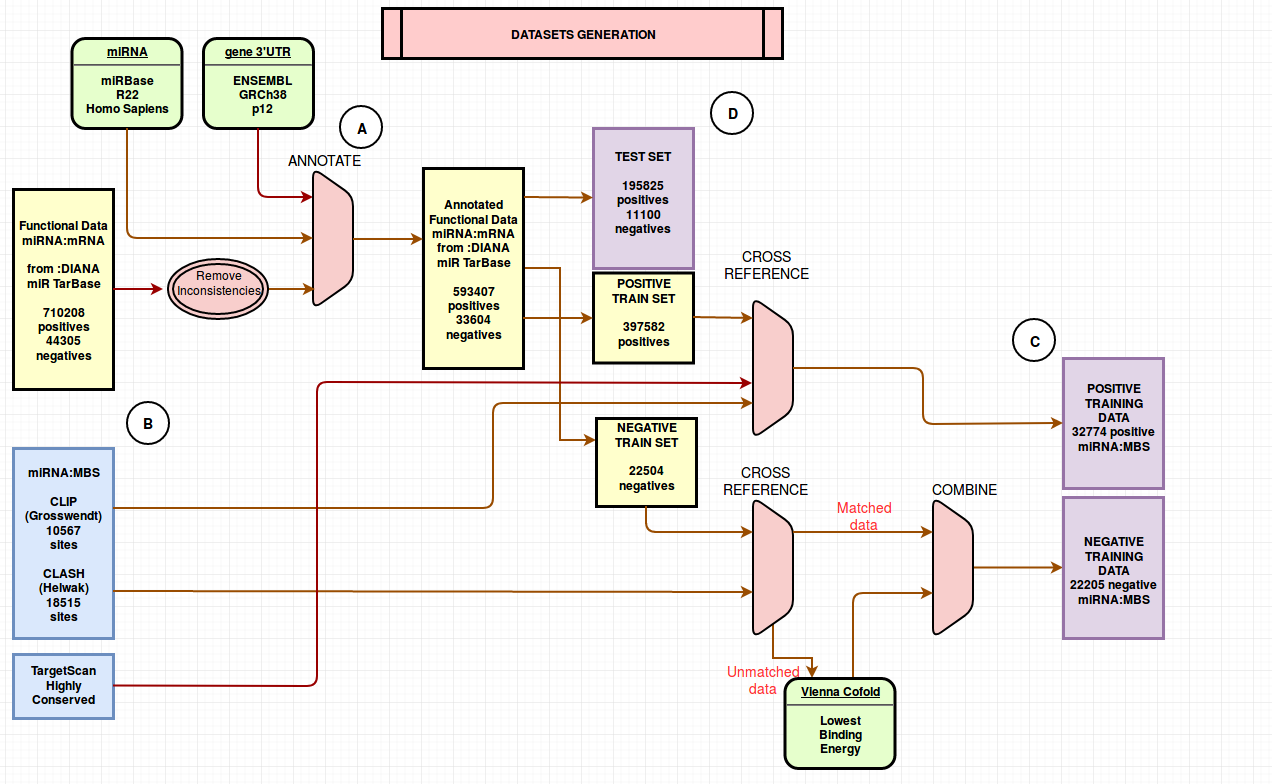
\includegraphics[width=1\textwidth]{Figures/training}
	\caption{\textbf{The datasets generation process.} Two types of data were used: (i) experimentally verified functional datasets that define if a miRNA targets a gene - in yellow - and (ii) CLIP datasets that define miRNA binding site locations in the 3'UTR of a gene - in light blue -. In purple the final test and training sets. (A) Diana and miR TarBase were used as the main source of data: after removing inconsistent and duplicated data we annotated it using the Ensembl and the miRBase databases and subsequently, we split it into test and training set. (B) Training data were cross-referenced with CLIP and CLASH validated data providing information about the actual binding site of functional targets. The positive set was then complemented using highly conserved MBS locations provided by TargetScan (C) In order to obtain a consistent set of negative data for the training phase, we selected the miRNA:MBS with the lowest binding energy from the negative train set. (D) The final test set was extracted keeping the 33\% of all available data.}
	\label{fig:training}
\end{figure}

\section{The testing stage}
There is a big difference regarding the procedure adopted for the testing stage compared to the training phase. Here the purpose is to predict if a given miRNA targets a certain gene, hence the testing data consists of pairs containing the miRNA and the whole 3'UTR transcript, rather than a specific MBS. This step is essential to be able to evaluate the whole pipeline process of DeepMiRNA.

To correctly evaluate the network performance we used the experimentally verified miRNA:mRNA pairs excluded from the training set. Those data points, however, were highly biased towards positive entries in a ratio of 95:5 and this imbalance could impede a true evaluation of the trained model. In fact, a tool that exclusively predicts positive targets against the full test data would achieve an accuracy of 95\%. 

Nevertheless, using suitable metrics, such as f1-score, precision and recall, as described in \cite{imbalanced}, is still possible to effectively overcome this issue.

\subsection{Candidate site selection methods: CSSM}
Often, in the academic world, people tend to affirm that, in order to properly train a neural network, one needs to have a huge amount of data available. While we partially disagree with this common belief, convinced that quality and variety prevail over quantity, we still agree that in the case of miRNA targets prediction the available experimentally validated data is still not sufficiently representative of the task and the candidate site selection step effectively narrows the search space to simplify the NN classification task.

For this reason, the selection of candidate sites in an mRNA becomes a key step for a miRNA target sites predictor because it helps to identify which regions within the mRNA have the potential to accommodate a binding site. We found out that most of the publicly available algorithms follow a similar approach: they scan the gene's 3'UTR  looking for sites that are partially complementary to the miRNA transcript; if a site meets certain criteria, it is considered to be a candidate site and is subjected to further analysis.

In the light of new recent results, stating that functional miRNA targets can arise either by a single strong binding site (i.e. 6 consecutive complementary nucleotides) or by multiple weak binding sites \cite{helwak}, we believe it's essential to consider the whole 3'UTR sequence using CSSM willing to accept both canonical and non-canonical sites. These methods are less conservative and allow accepting bulges, mismatches or wobble pairs in the seed region (see figure \ref{fig:canonical}).

\begin{figure}[hbt!]
	\centering
	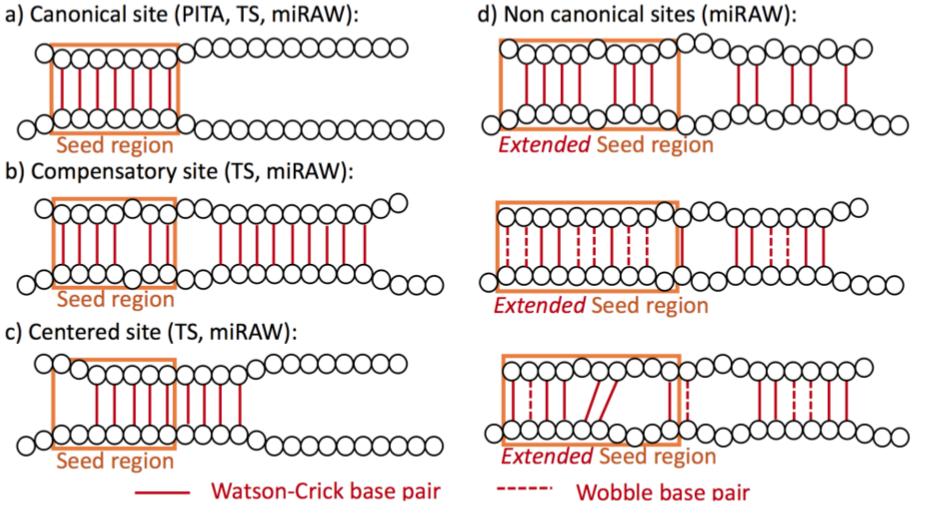
\includegraphics[width=1\textwidth]{Figures/canonical}
	\caption{Example of canonical and non-canonical sites used in three available tools: Pita, TargetScan and miRAW.}
	\label{fig:canonical}
\end{figure}

The CSSM adopted in DeepMiRNA use a very similar approach to miRAW \cite{miraw}: we consider a 30-nucleotide window to scan the 3'UTR and we extend the typical 7mer seed region (figure \ref{fig:canonical}a) considering the first 10 nucleotides of the miRNA transcript (figure \ref{fig:canonical}d) to look for partial complementarity.

In particular, we consider a site to be a potential candidate site if there is a minimum number of base pairs, both Watson-Crick and Wobble, within the extended seed region. In this thesis we investigated three different configurations: 

\begin{enumerate}
	\item CSS-6.0:10: a candidate site must contain at least 6 base pairs between the extended seed region composed of the first 10 nucleotides;
	\item CSS-7.0:10: a candidate site must contain at least 7 base pairs between the extended seed region composed of the first 10 nucleotides;
	\item CSS-7.1:10: a candidate site must contain at least 7 base pairs between the extended seed region composed of the 9 nucleotides comprised from the second and the tenth. 
	
\end{enumerate}

In each case, base pairs do not need to be consecutive in order to accommodate the presence of gaps and bulges. The task of finding non-consecutive complementary nucleotides can be mapped to the problem of finding the longest common subsequence (LCS ) between two strings as illustrated in figure \ref{fig:lcs}.

\begin{figure}[hbt!]
	\centering
	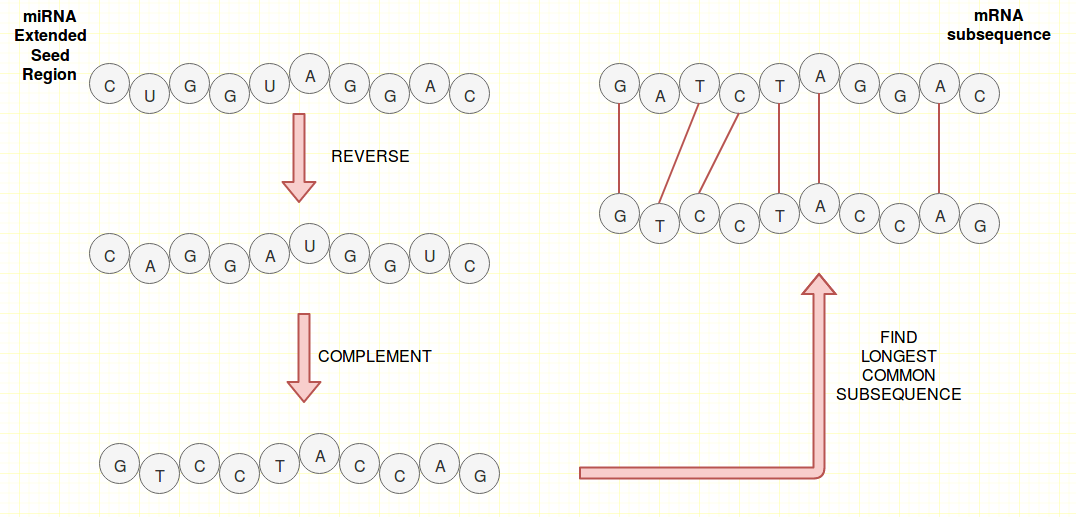
\includegraphics[width=1\textwidth]{Figures/lcs}
	\caption{Mapping partial non-consecutive complementarity to longest common subsequence search.}
	\label{fig:lcs}
\end{figure}

Those configurations accept both standard canonical MBSs as well as a broader
range of non-canonical target site structures including the vast majority of experimentally validated sites from Diana TarBase and CLIP/CLASH binding site
datasets. Moreover, while these relaxed conditions for the seed region generate a much larger number of candidate sites and potentially an increased quantity of false positives, the decision of whether a site represents a functional target is delegated to the neural network. This way, we ensure that minimal assumptions, and hence bias, are incorporated into the analysis. 

\subsection{Longest Common Subsequence implementation}
The computational cost of the testing stage is considerably higher than that of the training phase. The reasons lie mainly in the computation of the potential candidate sites, involving a check of complementarity and the calculation of the minimum free energy, and the cost of the filtering stage (see next section).    
While there is very little to do with the calculation of the interaction energy of the duplexes, which completely relies on the Vienna Cofold library, for the complementarity check we tried different approaches to reduce the computational cost.

As mentioned above the seek of non-consecutive complementary nucleotides between two sequences can be seen as a special case of the problem of finding the longest common subsequence (LCS) between two strings. 

The LCS version we implemented in this thesis is done using \emph{Cython}\cite{cython}. Cython is a programming language that can be seen as a superset of Python that aims to give C-like performances with code that is mostly written using native Python. 

In fact, Cython actually works by producing Python modules where the code, however, is first translated and compiled into C.

For this reason, the Cython code must, unlike Python, be compiled. This usually happens in two stages: 

\begin{itemize}
	\item a \emph{.pyx} file is compiled by Cython into a \emph{.c} file;
	\item the \emph{.c} file is then compiled to a \emph{.so} file which can be imported and used directly in any Python session. 
\end{itemize}   

The algorithm we implemented uses dynamic programming and has a worst-case cost of $\mathcal{O}(n \times m)$ where $n$ and $m$ are the length of the sequences. The main difference between the classical implementation, that works by thoroughly filling a $n \times m$ table and eventually uses  backtracking to recover the final result, and our approach, consists in how we handle the table construction. In fact, unlike the original implementation, we update the table only when a match is found, thus reducing the whole computational cost. 

However, for our task, we found out that the number of updates required is, on average, around 70\% of the table size. This is most likely due to the reduced alphabet size (four letters) of the sequences. For this reason, the total cost of the function is comparable with the regular implementation.

On average the Cython version of the algorithm is 20 times faster than the original Python implementation and this justifies its use in the DeepMiRNA pipeline.

      

\subsection{Filtering predictions} \label{sub:filtering_step}
In chapter \ref{Chapter3} we highlighted the importance of site accessibility for miRNA target prediction. In fact, many studies \cite{helwak} \cite{common_features} have proved genes accommodate site accessibility by preferentially positioning targets in highly accessible regions \cite{accessibility_nrg_role} thus demonstrating that target accessibility may be a useful feature.

Moreover, the use of a greedier CSSM approach may give rise to an increase in the number of potential candidate sites for each miRNA:mRNA duplex. For example, on average, where a strict canonical approach identifies $\approx$ 3-4 sites per duplex, CSS-6.0:10 identifies approximately 32 MBSs while CSS-7.0:10 about 21 and CSS-7.1:10 around 15. As a consequence, the chance of obtaining more false positives is very likely to increase.  

This could represent a problem for the neural network, because it may not be able to completely discern false from true positive duplexes. This could be due, in particular, to two main factors: first of all the number of validated negative MBSs is extremely low; in fact, despite having a good number of negative miRNA:mRNA pairs, we only have a small quantity of negatively validated binding sites. Thus, we had to artificially select the negative sites for the training stage as explained in the previous section. Second, functional and non-functional sites are very similar in terms of complementarity with the pairing miRNA and, hence, we believe it's important to also consider the characteristics of the secondary structure of the duplex to improve the accuracy of the prediction and reduce the number of false positives. 

To this purpose, we investigated the possibility of using an a-posteriori filter that considers the secondary structure and computes the site accessibility of the target site. The site accessibility has been computed as follows:
\begin{itemize}
	\item for each potential site identified using the CSSM, we considered the region of 200 nucleotides surrounding the MBS and we call it \emph{folding chunk}. For example, if the MBS has length 30 and comprises the region between nucleotide 100 and 129, we consider for the computation of the site accessibility the region between nucleotide 15 and 214. If either on the left or on the right-hand side of the MBS there were not enough nucleotides we considered a shorter fold;
	\item the free energy $\Delta G_{free}$ of the folding region is computed, using Vienna Cofold, to check the amount of energy released during the reaction;
	\item next we computed the opening energy $\Delta G_{open}$, that is the energy needed to unfold the mRNA and allow the miRNA binding;
	\item the site accessibility energy $\Delta\Delta G$ is given by the difference between the free energy released with the binding and the opening energy (see figure \ref{fig:site_accessibility}). The bigger the value the more accessible the site:
	\begin{equation} \label{eq:sa}
		\Delta\Delta G = \Delta G_{free} - \Delta G_{open}
	\end{equation}
	 
\end{itemize}    

In order to use this feature as a filter, we set a site accessibility threshold meaning that sites with a low value are discarded while only MBSs with site accessibility greater than the threshold are considered as functional. 

The use of the filtering stage has proved to be useful in case of more complex networks such as convolutional models, while for a simpler network such as the feed-forward model available in DeepMiRNA this feature did not provide any significant benefit.

In addition, one may wonder why we used this feature as an a-posteriori filter rather than using it as another candidate selection rule. While the final result is the same, computing the secondary structure of a folding chunk, and hence its accessibility, is a pretty difficult task involving a lot more computation than asking the network for a prediction. Thus, we decided to use this feature as the last pipeline step.

\begin{figure}[hbt!]
	\centering
	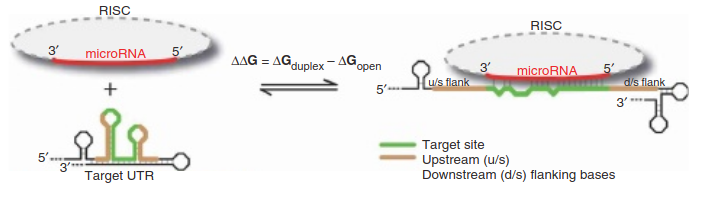
\includegraphics[width=1\textwidth]{Figures/site_accessibility}
	\caption{Illustration of site accessibility energy for miRNA:MBS interactions.}
	\label{fig:site_accessibility}
\end{figure}

\subsection{Obtaining the final classification} \label{sub:prediction}
In order to classify a given duplex, we consider that the miRNA targets a gene if any of the potential MBSs of the mRNA is predicted to be functional. The targeting process implemented in DeepMiRNA requires the neural network to classify at least one not filtered candidate site as functional to consider a miRNA:mRNA as a positive targeting event. 

More specifically, given a miRNA $m$, a gene $g$ and a free energy threshold for the duplex $th_{duplex}$, a candidate site selection method $sm(m,g, th_{duplex})$ determines a set $CS$ of potential MBSs, considering both partial complementarity and stability of the bond. 

For this last requirement we chose a threshold $th_{duplex} = -10kcal/mol$, meaning that only miRNA:MBS pairs with a free energy lower than this threshold are kept:
%
\begin{equation} \label{eq:eq1}
	sm(m,g, th_{duplex}) = CS
\end{equation}
% prevent blank line
To determine if the miRNA is targeting the gene, each candidate site within the miRNA:mRNA segment is properly encoded and input to the neural network. The result of the targeting prediction $T(m, g)$ corresponds to the disjunction of the conjunction between the neural network outputs for all the candidate sites and the site accessibility check:
%
\begin{equation} \label{eq:eq2}
	T(m,g) = \bigvee_{cs}{nn(m,cs) \wedge \Delta\Delta G(cs) > th_{sa}}
\end{equation} 
%
Where $nn(m,cs)$ denotes the output of the neural network while $\Delta\Delta G(cs) > th_{sa}$ represents the filtering step checking the site accessibility of the candidate is sufficiently high. When the filter is not used this term is always equal to $1$.

The best performance has been achieved by setting $th_{sa} = -14kcal/mol$.



